\begin{homeworkProblem}[2]
    Consider again the model of the medieval economy discussed in class: 
    
    \begin{enumerate}[topsep=15pt]
        \item[] \quad \quad \:\:\: $\log M_t + \log V = \log P_t + \log Y_t$
        \item[] \quad \quad \:\:\: $\log P_{t+1} - \log P_t = \theta (\log Y_t - \log Y^*)$
    \end{enumerate}

    We would like to rewrite the model in terms of inflation and the ``output
    gap"---i.e., the gap between actual output and steady state ouput. We denote
    inflation by $\pi_t$. Recall that inflation is defined as $\left( P_{t+1}-P_t \right)  /P_t$.
    For inflation rates close to zero the following approximation is quite accurate 
    $\pi_t \approx \log (1+\pi_t) = \log (P_t/P_{t-1})$. Please make use of this
    as needed in solving the problem. We denote the output gap by $\Tilde{Y_t}= \log Y_t - \log Y^*$.
    \\ \\
    A) Using this notation, show that the medieval economy model can be rewritten
    as:
    
    \begin{flalign*}
        & \quad \quad \text{AD:} \quad \quad \Delta \log M_t = \pi_t + \widetilde{Y_t} - \widetilde{Y}_{t-1} &\\
        & \quad \quad \text{SRAS:} \quad \pi_t = \theta \widetilde{Y}_{t-1} &\\
    \end{flalign*}

    
    where AD stands for ``aggregate demand" and SRAS stands for ``short-run 
    aggregate supply." These labels will be explained in class.
    \\ \\ \\
    In the simplest version of the medieval economy, the money supply is
    exogenously given by, say, the number of gold coins in the economy. 
    Suppose now that the government starts issuing paper money and can thus
    change the supply of the money at will. For simplicity, suppose the 
    economy is in a steady state with zero inflation at time 0. In other 
    words, $\pi_0 = 0$ and $\widetilde{Y}_0 = 0$. Also, assume that $\theta = 0.25$. 
    \\ \\
    B) By an unfortunate turn of events, a crazy person takes over as the 
    chairman of the central bank in our medieval economy with paper money. 
    Suppose this person decides to raise the money supply by one log unit 
    every odd period and reduce it by one log unit every even period. In
    other words $\Delta \log M_t = 1$ in odd periods and $\Delta \log M_t
    = -1$ in even periods. Solve for the dynamics of the output gap and
    inflation for 20 periods in this case.
    \\ \\
    C) The dynamics that come out of part (b) may strike you as strange. 
    Do, you think this is actually what would happen if such a crazy 
    person were to take over at the central bank? Remember that the logic
    of the model is that the reason why output deviates from desired output
    is that producers are surprised by changes in the stock of money. We 
    motivated this assumption by the notion that in the medieval economy 
    without paper money the money supply rarely changed and any changes 
    were true surprises. Remembering that the producers are trying to 
    achieve a zero output gap, explain how their behavior may eventually 
    differ from the behavior embodied in the SRAS equation above.
    \\ \\
    Now suppose that the crazy central banker is thrown out of office 
    (this is not the answer I am looking for in part C)) and the money 
    supply doesn’t change for a while so that economy again settles 
    down to the steady state with zero inflation. At that point, a new 
    central banker is hired and (s)he decides to start steadily increasing 
    the money supply. More specifically, suppose the money supply grows 
    at a constant rate $\Delta \log M_t = \Delta \log M$.
    \\ \\
    D) Assuming that the behavior of the people in the economy is well
    described by the AD and SRAS equations above, what is the steady 
    state value of the output gap and inflation for this economy as a 
    function of $\Delta \log M$?
    \\ \\
    E) Again assuming that the behavior of the people in the economy 
    is well described by the AD and SRAS equations above, plot the 
    relationship between steady state inflation and the steady state 
    output gap for different constant values of money growth with 
    inflation on the vertical axis and the output gap on the horizontal 
    axis. We refer to this relationship as the “long run aggregate supply” 
    (LRAS) relationship in the medieval model.
    \\ \\
    F) The following quote is attributed to Abraham Lincoln: “You can 
    fool some of the people all of the time, and all of the people some 
    of the time, but you cannot fool all of the people all of the time.” 
    Discuss the realism of the price setting behavior that underlies the
    SRAS curve in light of the LRAS curve derived above and Lincoln’s quote.

    \pagebreak
    \part

    Show that the medieval economy model can be rewritten as:
    
    \begin{flalign*}
        & \quad \quad \text{AD:} \quad \quad \Delta \log M_t = \pi_t + \widetilde{Y_t} - \widetilde{Y}_{t-1} &\\
        & \quad \quad \text{SRAS:} \quad \pi_t = \theta \widetilde{Y}_{t-1} &\\
    \end{flalign*}

    
    where AD stands for ``aggregate demand" and SRAS stands for ``short-run 
    aggregate supply." These labels will be explained in class.    
    \\ \\
    \solution
    \\
    First, I will derive the equation for aggregate demand using the
    first equation by taking a difference in the logarithm of the
    money supply between time $t$ and $t-1$

    \[
        \begin{split}
            \log M_t + \log V &= \log P_t + \log Y_t
            \\
            \log M_t &= \log P_t + \log Y_t - \log V
            \\
            \log M_{t} - \log M_{t-1} &= \log P_{t} - \log P_{t-1} + \log Y_{t} - \log Y_{t-1}
            \\
            \Delta \log M_t &= \log \frac{P_{t}}{P_{t-1}} + \log Y_{t} - \log Y^* - (\log Y_{t-1} - \log Y^*)
            \\
            \Delta \log M_t &= \pi_t + \widetilde{Y}_t -\widetilde{Y}_{t-1}
        \end{split}
    \]

    For short-run aggregate supply, I will reindex the second equation
    given in the specification and rewrite for inflation as a function
    of the output gap

    \[
        \begin{split}
            \log P_{t+1} - \log P_t &= \theta (\log Y_t - \log Y^*)
            \\
            \log P_t - \log P_{t-1} &= \theta (\log Y_{t-1} - \log Y^*)
            \\
            \log \frac{P_t}{P_{t-1}} &= \theta (\widetilde{Y}_{t-1})
            \\
            \pi_t &= \theta \widetilde{Y}_{t-1}
        \end{split}
    \]

    \pagebreak
    \part

    By an unfortunate turn of events, a crazy person takes over as the 
    chairman of the central bank in our medieval economy with paper money. 
    Suppose this person decides to raise the money supply by one log unit 
    every odd period and reduce it by one log unit every even period. In
    other words $\Delta \log M_t = 1$ in odd periods and $\Delta \log M_t
    = -1$ in even periods. Solve for the dynamics of the output gap and
    inflation for 20 periods in this case.
    \\ \\
    \solution 

    To solve for the output gap and inflation across these 20 time periods,
    I will rewrite the aggregate demand equation in terms of the output gap
    and then plot the log money supply, the output gap, and inflation over
    time
    \[
        \begin{split}
            \Delta \log M_t &= \pi_t + \widetilde{Y}_t -\widetilde{Y}_{t-1}
            \\
            \widetilde{Y}_t &= \Delta \log M_t - \pi_t + \widetilde{Y}_{t-1}
        \end{split}
    \]

    Given that the log money supply, the output gap, and inflation all start
    at zero, below is a plot of their dynamics over 20 time periods when
    $\theta$ is equal to 0.25

    \begin{figure}[h]
        \centering
        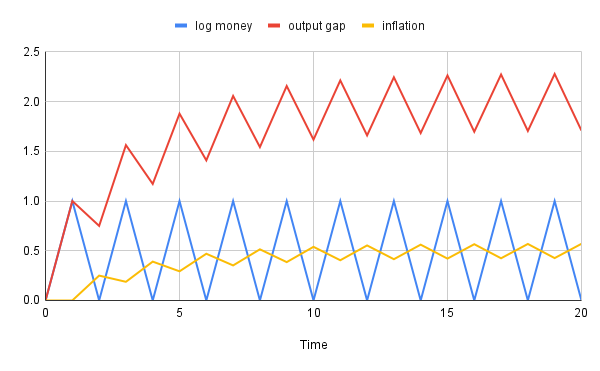
\includegraphics[width=1\linewidth]{crazy.png}
        % \caption{Caption}
        \label{fig:enter-label}
    \end{figure}

    \pagebreak
    \part

    The dynamics that come out of part (b) may strike you as strange. 
    Do, you think this is actually what would happen if such a crazy 
    person were to take over at the central bank? Remember that the logic
    of the model is that the reason why output deviates from desired output
    is that producers are surprised by changes in the stock of money. We 
    motivated this assumption by the notion that in the medieval economy 
    without paper money the money supply rarely changed and any changes 
    were true surprises. Remembering that the producers are trying to 
    achieve a zero output gap, explain how their behavior may eventually 
    differ from the behavior embodied in the SRAS equation above.
    \\ \\
    \solution

    Since the element of suprise is lost from the increased demand 
    due to the predictable changes in the money supply by the crazy
    central banker, producers will eventually figure out how to adjust 
    their expectations and prices accordingly, with a forecast of the 
    periodic jumps and falls in the money supply. This will close the 
    output gap as prices rein in the increased demand from the money 
    supply, returning output to $Y^*$. 

    \pagebreak
    \part 

    Now suppose that the crazy central banker is thrown out of office 
    (this is not the answer I am looking for in part C)) and the money 
    supply doesn’t change for a while so that economy again settles 
    down to the steady state with zero inflation. At that point, a new 
    central banker is hired and (s)he decides to start steadily increasing 
    the money supply. More specifically, suppose the money supply grows 
    at a constant rate $\Delta \log M_t = \Delta \log M$.
    \\ \\
    Assuming that the behavior of the people in the economy is well
    described by the AD and SRAS equations above, what is the steady 
    state value of the output gap and inflation for this economy as a 
    function of $\Delta \log M$?
    \\ \\
    \solution 

    In a steady state, time-dependent variables don't change across
    time periods, so $\widetilde{Y}_t = \widetilde{Y}_{t-1}$, and if
    we know that the money supply grows at a constant rate, we can 
    substitute int our aggregate demand and short-run aggregate supply
    equations

    \[
        \begin{split}
            \Delta \log M_t &= \pi_t + \widetilde{Y}_t - \widetilde{Y}_{t-1}
            \\
            \Delta \log M &= \pi + \widetilde{Y} - \widetilde{Y}
            \\
            \Delta \log M &= \pi
        \end{split}
    \]

    And now using our short-run aggregate supply equation to solve for
    the output gap, substituting in $\Delta \log M$ in for inflation $\pi$

    \[
        \begin{split}
            \pi_t &= \theta \widetilde{Y}_{t-1}
            \\
            \pi &= \theta \widetilde{Y}
            \\
            \log M &= \theta \widetilde{Y}
            \\
            \frac{\log M}{\theta} &= \widetilde{Y}
        \end{split}
    \]
    
    \pagebreak
    \part

    Again assuming that the behavior of the people in the economy 
    is well described by the AD and SRAS equations above, plot the 
    relationship between steady state inflation and the steady state 
    output gap for different constant values of money growth with 
    inflation on the vertical axis and the output gap on the horizontal 
    axis. We refer to this relationship as the “long run aggregate supply” 
    (LRAS) relationship in the medieval model.
    \\ \\
    \solution 
    
    Below is a plot of steady state inflation over steady state output gap,
    relating the two across many different growths of the money supply. The
    plot is linear, with a slope of $d\pi / d\widetilde{Y} = \theta$
    \\
    \begin{center}
        \begin{tikzpicture}
            \begin{axis}[standard,
                    ytick=\empty,
                    xtick=\empty,
                    xticklabels={},
                    yticklabels={},
                    xlabel={Output gap $\widetilde{Y}$},
                    ylabel={Inflation $\pi$},
                    samples=1000, 
                    xmin=0,
                    xmax=5,
                    ymin=0,
                    ymax=5]
                \addplot[line width=0.8mm,red,domain={0:5}]{0.75*x};
            \end{axis}
        \end{tikzpicture}      
    \end{center}

    \pagebreak
    \part 

    The following quote is attributed to Abraham Lincoln: “You can 
    fool some of the people all of the time, and all of the people some 
    of the time, but you cannot fool all of the people all of the time.” 
    Discuss the realism of the price setting behavior that underlies the
    SRAS curve in light of the LRAS curve derived above and Lincoln’s quote.
    \\ \\
    \solution 

    The quote in the context of our discussion highlights the short-run nature
    of increased output due to monetary policy. Although with some constant
    inflation it is possible to maintain an output gap, in the long run, steady
    state output is not determined by the money supply in an economy. And if
    prices were able to adjust instantly to the money supply, it would be impossible
    to maintain elevated output by tweaking the money supply.
    
\end{homeworkProblem}